\documentclass[aspectratio=169]{beamer}
\usepackage[utf8]{inputenc}
\usepackage[T1]{fontenc}
\usepackage[brazilian,provide=*]{babel}
\usepackage{booktabs}
\usepackage{array}
\usepackage{graphicx}
\graphicspath{{img/}{./}}
\usepackage{tikz}
\usetikzlibrary{positioning, shapes.geometric, arrows}
\usetheme{Madrid}
\definecolor{pucazul}{RGB}{0,45,98}
\definecolor{okverde}{RGB}{25,135,84}
\definecolor{falhavermelho}{RGB}{176,32,32}
\usecolortheme[named=pucazul]{structure}
\setbeamercolor{title}{fg=white,bg=pucazul}
\setbeamercolor{frametitle}{fg=white,bg=pucazul}
\setbeamercolor{block title}{fg=white,bg=pucazul}
\setbeamercolor{block title alerted}{fg=white,bg=red!70!black}
\setbeamercolor{block title example}{fg=white,bg=green!40!black}
\setbeamertemplate{navigation symbols}{}
\addtobeamertemplate{frametitle}{}{%
  \begin{tikzpicture}[remember picture,overlay]
    \node[anchor=north east, inner sep=0pt, xshift=-3mm, yshift=-1.5mm] at (current page.north east)
      {
\includegraphics[height=0.9cm,width=2.6cm,keepaspectratio]{logo_puc.png}};
  \end{tikzpicture}}
\newcommand{\caixa}[2]{\parbox[t][#1][t]{\linewidth}{\raggedright #2}}
\newcommand{\ok}{\textcolor{okverde}{\textbf{Aprovado}}}
\newcommand{\falha}{\textcolor{falhavermelho}{\textbf{Reprovado}}}
\setbeamertemplate{footline}{
  \leavevmode%
  \hbox{%
  \begin{beamercolorbox}[wd=.333333\paperwidth,ht=2.25ex,dp=1ex,center]{author in head/foot}%
    \usebeamerfont{author in head/foot}Projeto de Testes -- Sistema de RH
  \end{beamercolorbox}%
  \begin{beamercolorbox}[wd=.333333\paperwidth,ht=2.25ex,dp=1ex,center]{title in head/foot}%
    \usebeamerfont{title in head/foot}PUC Minas Betim
  \end{beamercolorbox}%
  \begin{beamercolorbox}[wd=.333333\paperwidth,ht=2.25ex,dp=1ex,right]{date in head/foot}%
    \usebeamerfont{date in head/foot}\insertshortdate{}\hspace*{2em}
    \insertframenumber{} / \inserttotalframenumber\hspace*{2ex}
  \end{beamercolorbox}}%
}
\title[Projeto de Testes]{Projeto de Testes: Sistema de RH ``Me Contrate''}
\subtitle{Teste e Manutenção de Software}
\author[Grupo]{\footnotesize
  \begin{tabular}{cc}
    Arthur Souza Carvalho & Gustavo Rodrigues de Almeida \\
    Marlon Magalhaes Carvalho & Moises Samuel Rezende Maia \\
    Otavio Nascimento de Castro & Sarah Palhares Araujo
  \end{tabular}}
\institute[PUC Minas Betim]{Sistemas de Informação \\ PUC Minas Betim}
\date{Novembro de 2026}
\titlegraphic{
\includegraphics[height=1.3cm]{logo_puc_azul.png}}
\hypersetup{pdftitle={Projeto de Testes: Sistema de RH Me Contrate}, pdfauthor={Arthur Souza Carvalho, Gustavo Rodrigues de Almeida, Marlon Magalhaes Carvalho, Moises Samuel Rezende Maia, Otavio Nascimento de Castro, Sarah Palhares Araujo}}

\begin{document}

% =====================================================================
% OTAVIO -- Capa, roteiro, sistema testado e plano (~2,5 min)
% =====================================================================

\begin{frame}[plain]
  \titlepage
\end{frame}

\begin{frame}{Roteiro}{Como vamos apresentar}
  \large
  \begin{enumerate}
    \setlength{\itemsep}{2.5mm}
    \item O sistema testado e o plano de testes
    \item Testes de unidade (Jest)
    \item Testes funcionais automatizados (Selenium)
    \item Refatoração de 2 métodos
    \item Testes manuais e relatório de defeitos
  \end{enumerate}
\end{frame}

\begin{frame}{O Sistema Testado}{TI ``Me Contrate'' -- Sistema de RH (2024/2)}
  \begin{columns}[c,onlytextwidth]
    \begin{column}{0.44\textwidth}
      \begin{block}{O que o sistema faz}
        \small
        \begin{itemize}
          \item Empresas se cadastram e \textbf{publicam vagas}.
          \item Candidatos se cadastram, \textbf{buscam vagas} e marcam ``Me Interessei''.
          \item Consulta pública de vagas e de candidatos.
        \end{itemize}
      \end{block}
      \small
      \textbf{Tecnologia:} HTML, CSS, JavaScript e Bootstrap.\\
      \textbf{Sem servidor:} tudo fica no \texttt{localStorage}.
    \end{column}
    \hfill
    \begin{column}{0.53\textwidth}
      \centering
      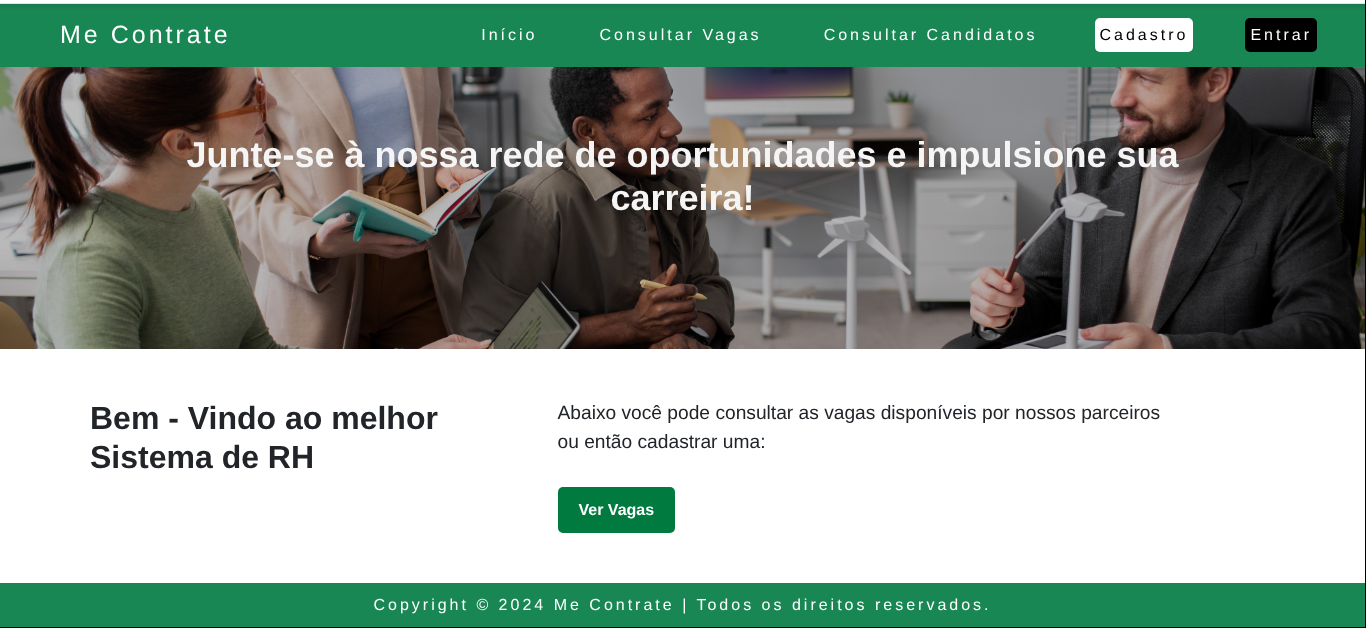
\includegraphics[width=\textwidth]{home.png}
    \end{column}
  \end{columns}
\end{frame}

\begin{frame}{Plano de Testes}{30 casos, 3 técnicas, 1 repositório}
  \begin{columns}[T,onlytextwidth]
    \begin{column}{0.31\textwidth}
      \begin{block}{Unidade}
        \small\caixa{2.3cm}{\textbf{10 casos} (CT01--CT10)\\Jest + jsdom\\Funções JavaScript originais do TI}
      \end{block}
    \end{column}
    \hfill
    \begin{column}{0.31\textwidth}
      \begin{block}{Automatizados}
        \small\caixa{2.3cm}{\textbf{10 casos} (CT11--CT20)\\Selenium WebDriver\\Google Chrome real}
      \end{block}
    \end{column}
    \hfill
    \begin{column}{0.31\textwidth}
      \begin{block}{Manuais}
        \small\caixa{2.3cm}{\textbf{10 casos} (CT21--CT30)\\Roteiro passo a passo\\Registro com prints}
      \end{block}
    \end{column}
  \end{columns}
  \vspace{3mm}
  \small
  \begin{itemize}
    \item \textbf{Escopo:} login, cadastros, vagas, candidatos, perfil, controle de acesso e responsividade.
    \item \textbf{Fora do escopo:} RF-05 a RF-10, que não foram implementados no TI.
    \item \textbf{Execução:} \texttt{npm install} e depois \texttt{npm test}.
  \end{itemize}
\end{frame}

% =====================================================================
% ARTHUR -- Testes de unidade CT01 a CT05 (~2 min)
% =====================================================================

\begin{frame}{Testes de Unidade}{Como testamos o código original sem alterá-lo}
  \begin{columns}[c,onlytextwidth]
    \begin{column}{0.40\textwidth}
      \small
      \begin{enumerate}
        \setlength{\itemsep}{2mm}
        \item O teste carrega a \textbf{página HTML real} no jsdom.
        \item Executa o \textbf{arquivo .js original} do TI.
        \item Chama a função e confere o retorno, o \texttt{localStorage} e os alertas.
      \end{enumerate}
      \vspace{2mm}
      \begin{exampleblock}{CT01 a CT05}
        \small Login de empresa e candidato, senha errada, e-mail inválido e nome curto: \textbf{5 aprovados}.
      \end{exampleblock}
    \end{column}
    \hfill
    \begin{column}{0.57\textwidth}
      \centering
      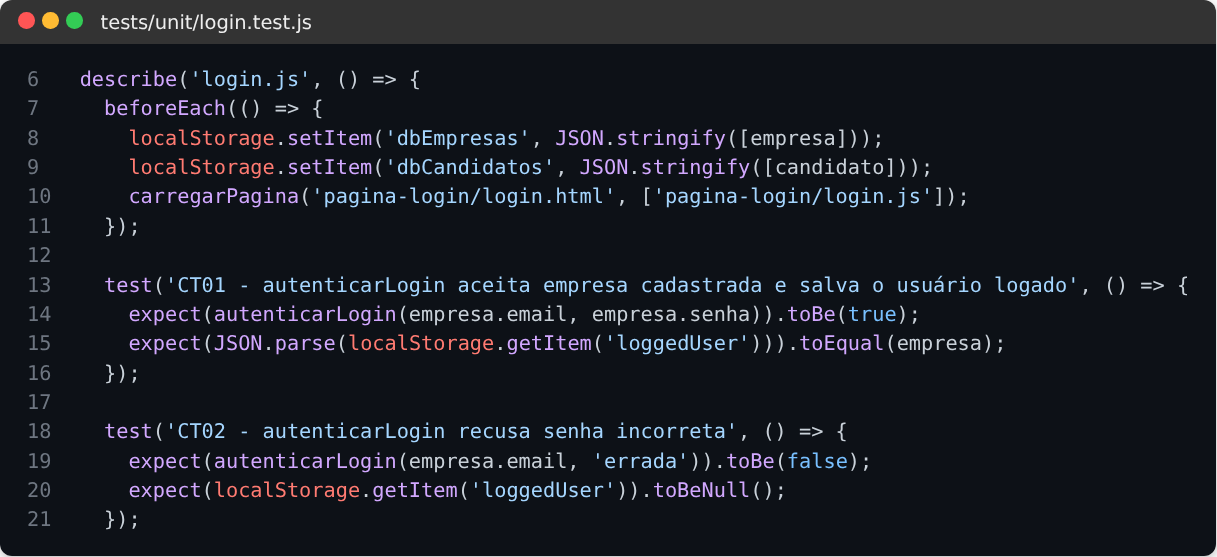
\includegraphics[width=\textwidth]{s_unit_codigo.png}
    \end{column}
  \end{columns}
\end{frame}

% =====================================================================
% GUSTAVO -- Testes de unidade CT06 a CT10 e falhas (~2 min)
% =====================================================================

\begin{frame}{Testes de Unidade}{Resultado: 8 aprovados e 2 reprovados}
  \begin{columns}[c,onlytextwidth]
    \begin{column}{0.47\textwidth}
      \centering
      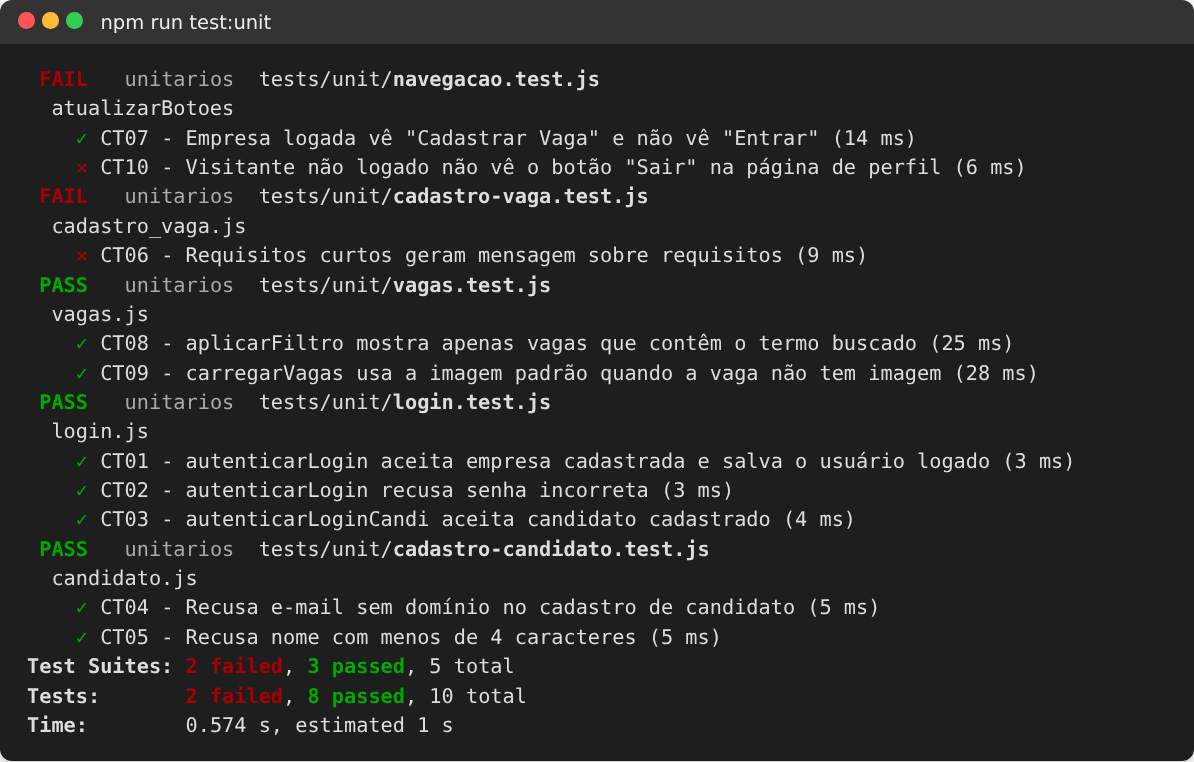
\includegraphics[width=\textwidth]{suite_unitarios.png}
    \end{column}
    \hfill
    \begin{column}{0.50\textwidth}
      \small
      \begin{alertblock}{CT06 -- Mensagem errada}
        \small Requisitos curtos geram o aviso ``O \textbf{contato} deve ter pelo menos 6 caracteres''.
      \end{alertblock}
      \begin{alertblock}{CT10 -- Função quebrada}
        \small \texttt{atualizarBotoes} do perfil usa a classe \texttt{"d-ne oone"} e lança exceção.
      \end{alertblock}
      CT07 a CT09 (menu, busca e imagem padrão): \ok.
    \end{column}
  \end{columns}
\end{frame}

% =====================================================================
% MARLON -- Selenium CT11 a CT16 (~2 min)
% =====================================================================

\begin{frame}{Testes Automatizados com Selenium}{Como a suíte funciona}
  \begin{columns}[c,onlytextwidth]
    \begin{column}{0.42\textwidth}
      \small
      \begin{itemize}
        \setlength{\itemsep}{2mm}
        \item A suíte sobe um \textbf{servidor local} com o código do TI.
        \item O Selenium abre o \textbf{Chrome} e limpa o \texttt{localStorage} antes de cada caso.
        \item Funções reutilizáveis: \texttt{fazerLogin}, \texttt{cadastrarVaga}, \texttt{aceitarAlerta}.
      \end{itemize}
      \begin{exampleblock}{CT11 a CT16}
        \small Cadastro de candidato e empresa, senhas diferentes e login: \textbf{6 aprovados}.
      \end{exampleblock}
    \end{column}
    \hfill
    \begin{column}{0.55\textwidth}
      \centering
      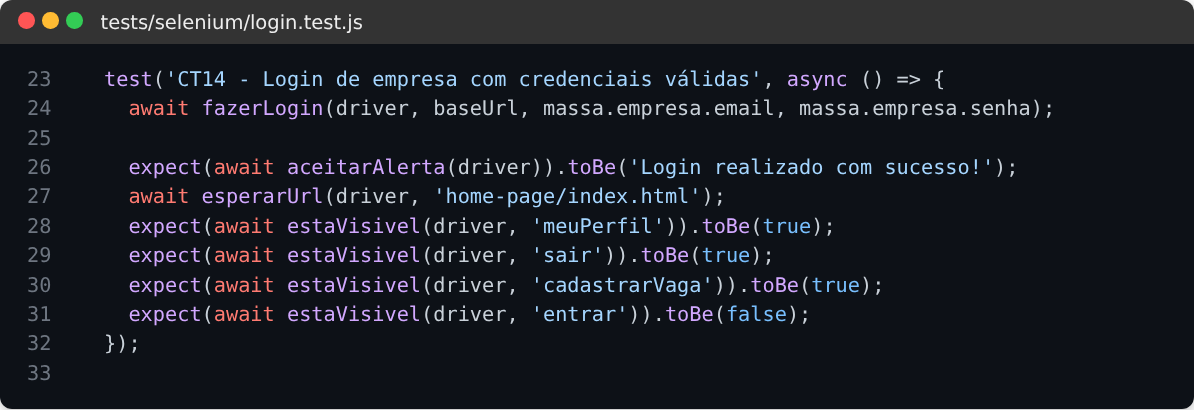
\includegraphics[width=\textwidth]{s_sel_codigo.png}
    \end{column}
  \end{columns}
\end{frame}

% =====================================================================
% MOISES -- Selenium CT17 a CT20 e refatorações (~3 min)
% =====================================================================

\begin{frame}{Testes Automatizados com Selenium}{Resultado: 9 aprovados e 1 reprovado}
  \begin{columns}[c,onlytextwidth]
    \begin{column}{0.48\textwidth}
      \centering
      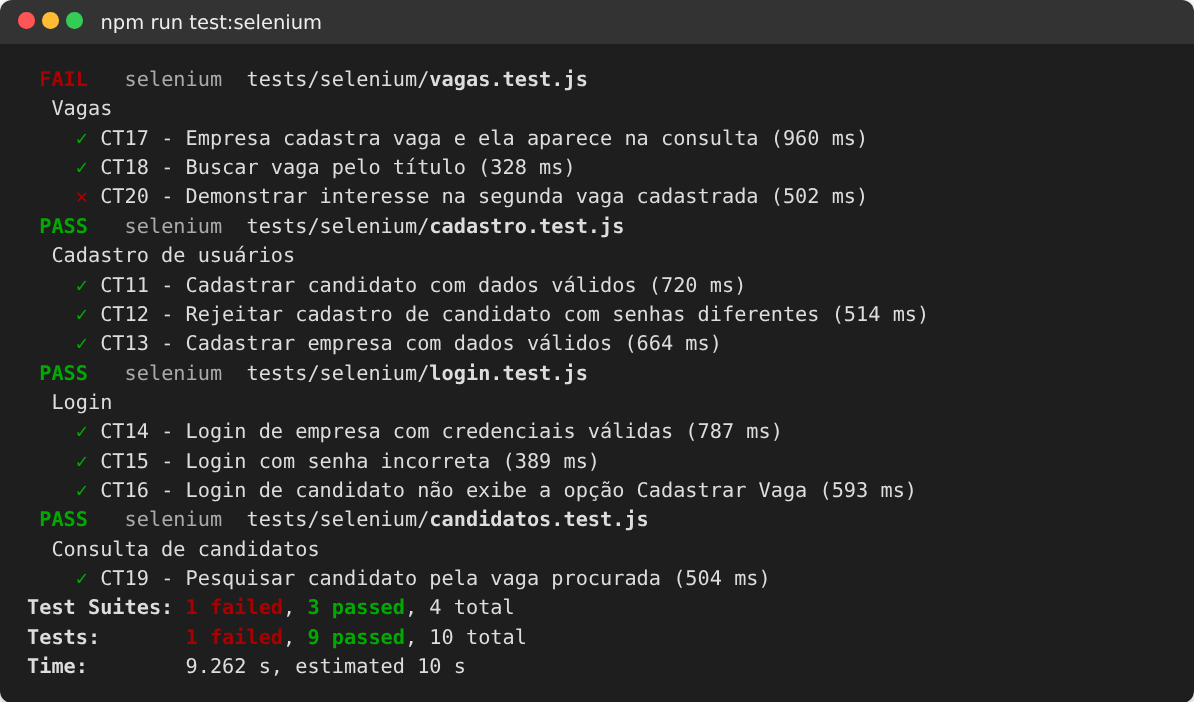
\includegraphics[width=\textwidth]{suite_selenium.png}
    \end{column}
    \hfill
    \begin{column}{0.49\textwidth}
      \small
      CT17 a CT19 (cadastrar vaga, buscar vaga e pesquisar candidato): \ok.
      \vspace{2mm}
      \begin{alertblock}{CT20 -- Interesse na vaga errada}
        \small Toda vaga cadastrada recebe o id \texttt{"vagaundefined"}. O interesse marcado na \textbf{2ª vaga} vai para a \textbf{1ª}.
      \end{alertblock}
    \end{column}
  \end{columns}
\end{frame}

\begin{frame}{Refatoração 1}{\texttt{realizarLogin} -- login.js}
  \begin{columns}[T,onlytextwidth]
    \begin{column}{0.49\textwidth}
      \centering
      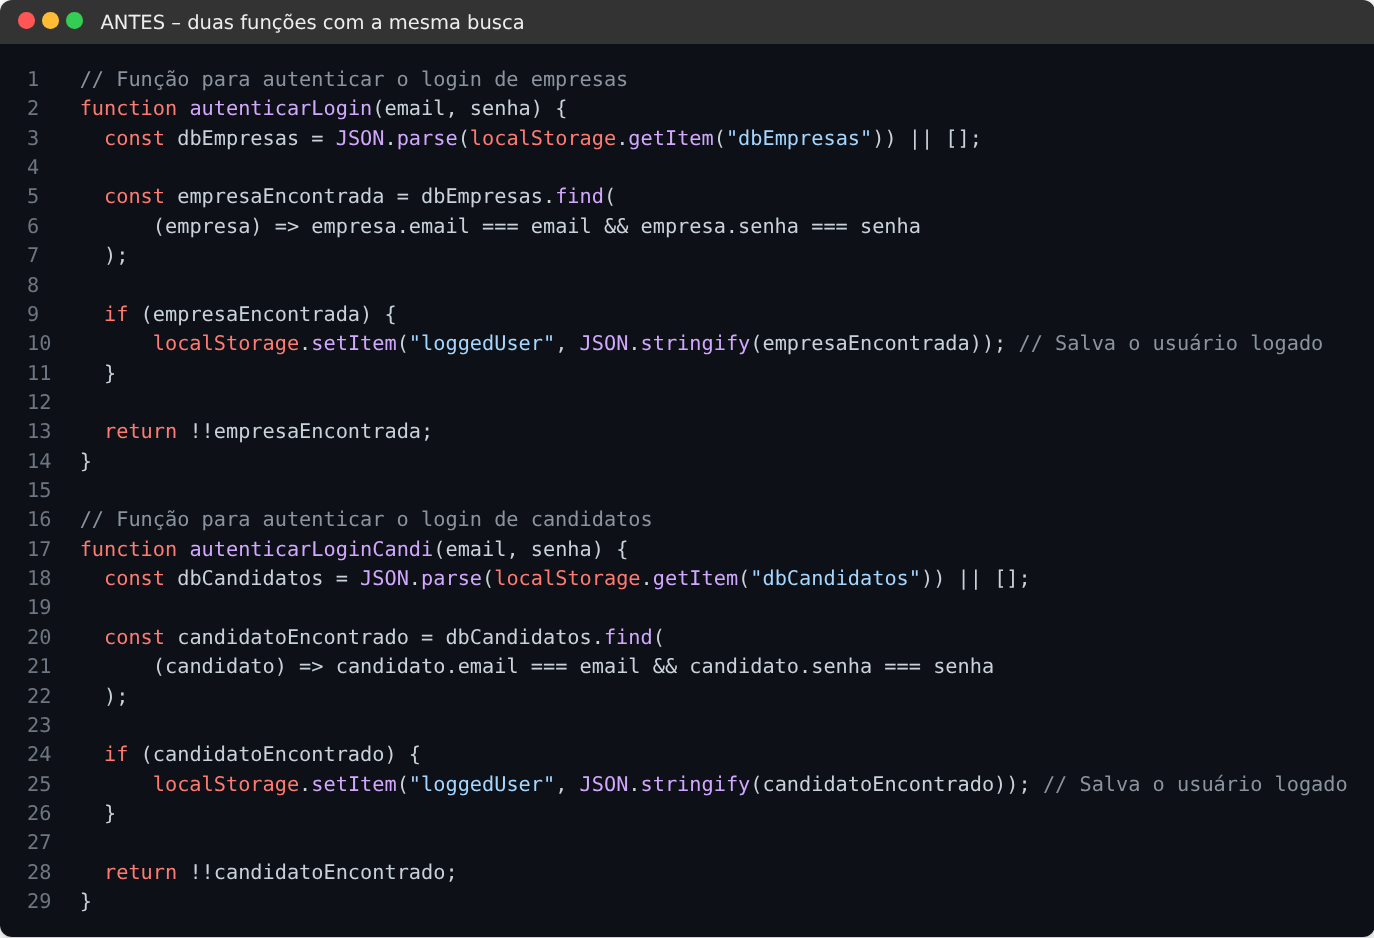
\includegraphics[width=\textwidth,height=6.6cm,keepaspectratio]{s_ref1_antes.png}
    \end{column}
    \hfill
    \begin{column}{0.49\textwidth}
      \centering
      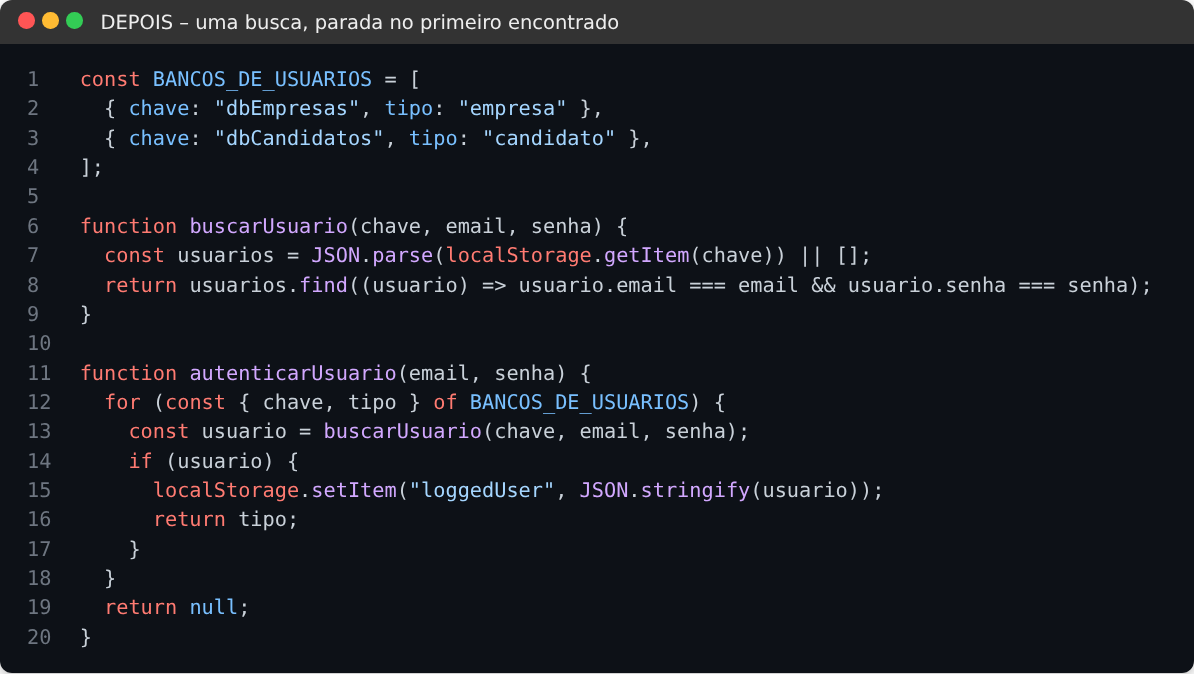
\includegraphics[width=0.9\textwidth]{s_ref1_depois.png}
      \vspace{1mm}
      \scriptsize
      \begin{itemize}
        \item \textbf{Extrair Método} (\texttt{buscarUsuario}) e \textbf{tabela de dados}.
        \item 61 $\rightarrow$ 41 linhas, sem busca duplicada.
        \item Corrige o login com o mesmo e-mail nas duas bases (D09).
      \end{itemize}
    \end{column}
  \end{columns}
\end{frame}

\begin{frame}{Refatoração 2}{\texttt{atualizarBotoes} -- telaperfil.js}
  \begin{columns}[T,onlytextwidth]
    \begin{column}{0.49\textwidth}
      \centering
      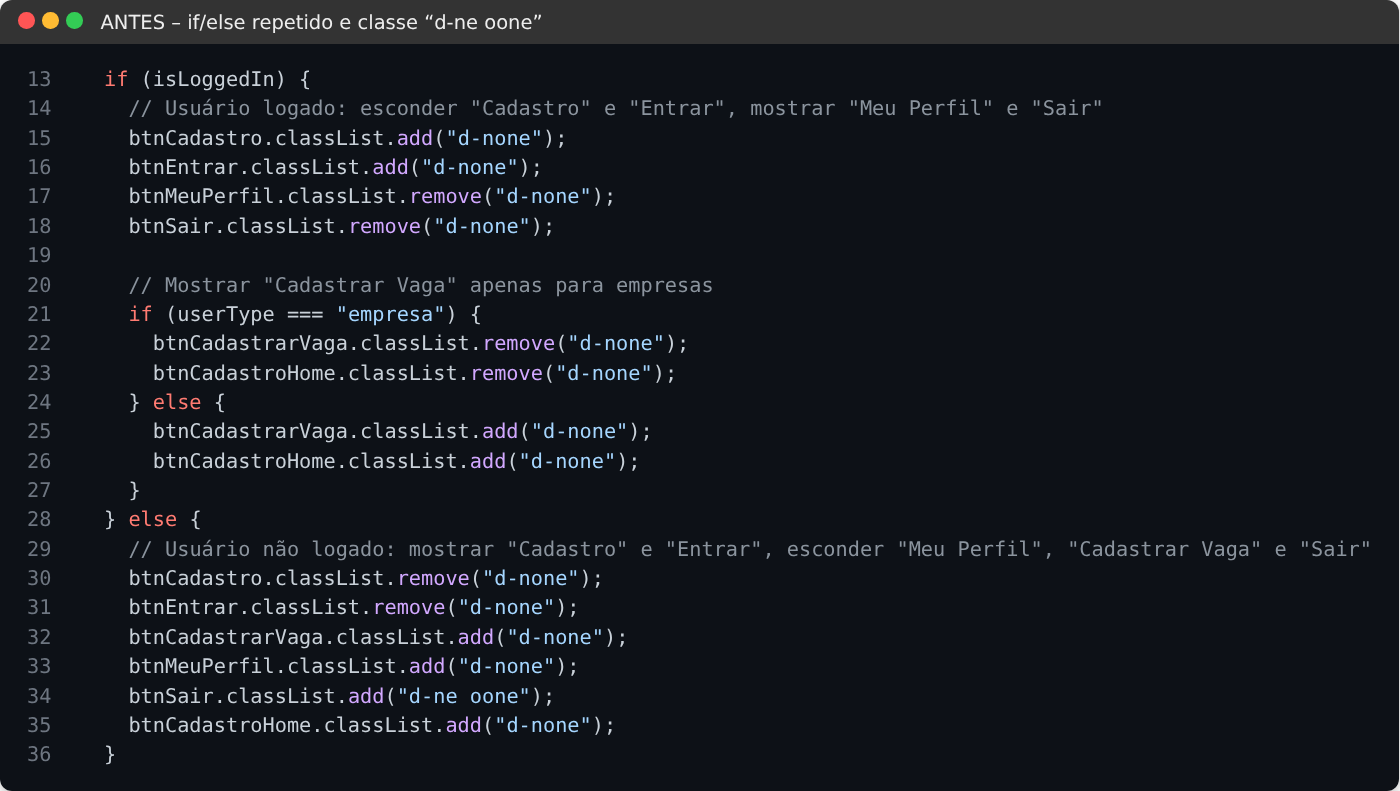
\includegraphics[width=\textwidth]{s_ref2_antes.png}
    \end{column}
    \hfill
    \begin{column}{0.49\textwidth}
      \centering
      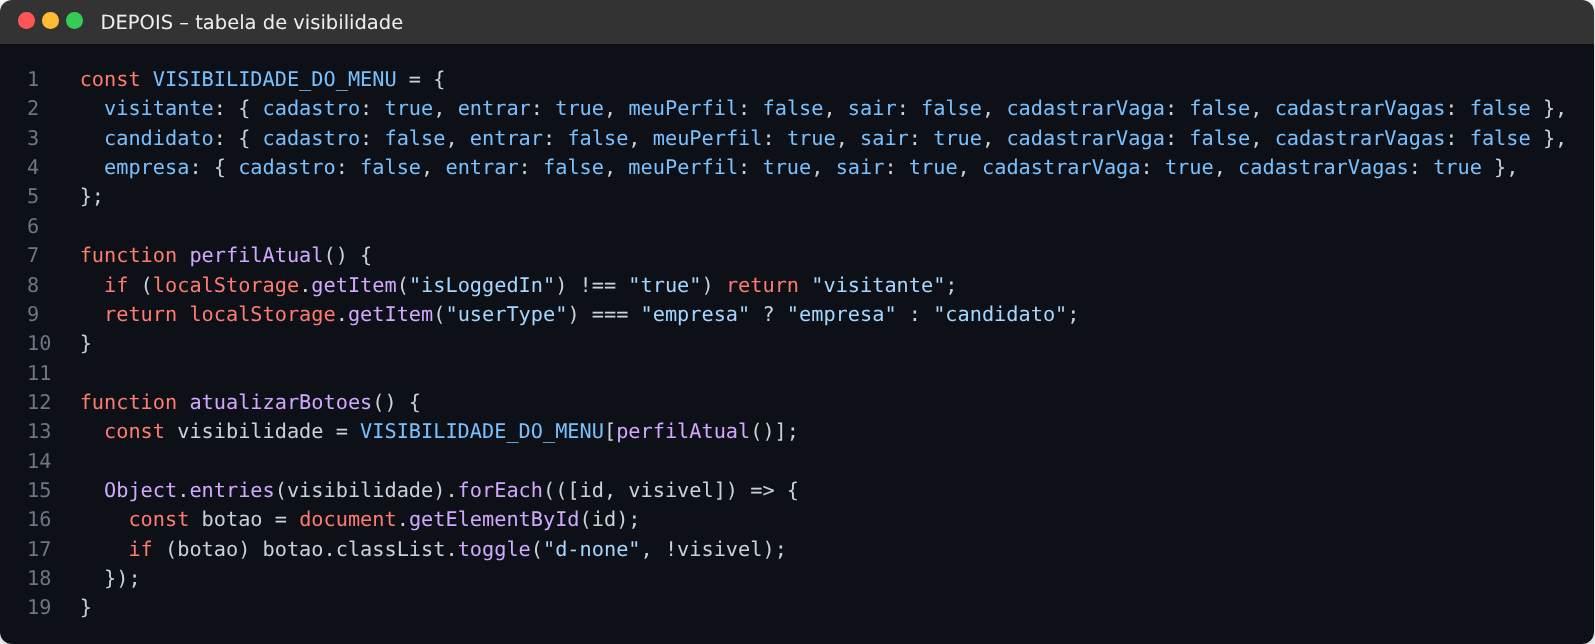
\includegraphics[width=\textwidth]{s_ref2_depois.png}
      \vspace{1mm}
      \scriptsize
      \begin{itemize}
        \item \textbf{Condicional $\rightarrow$ tabela} de visibilidade do menu.
        \item 37 $\rightarrow$ 19 linhas e corrige o defeito do CT10.
        \item 6 testes provam que o comportamento foi mantido.
      \end{itemize}
    \end{column}
  \end{columns}
\end{frame}

% =====================================================================
% SARAH -- Testes manuais, defeitos e conclusão (~3 min)
% =====================================================================

\begin{frame}{Testes Manuais}{10 casos com registro de prints: 6 aprovados e 4 reprovados}
  \begin{columns}[T,onlytextwidth]
    \begin{column}{0.49\textwidth}
      \centering
      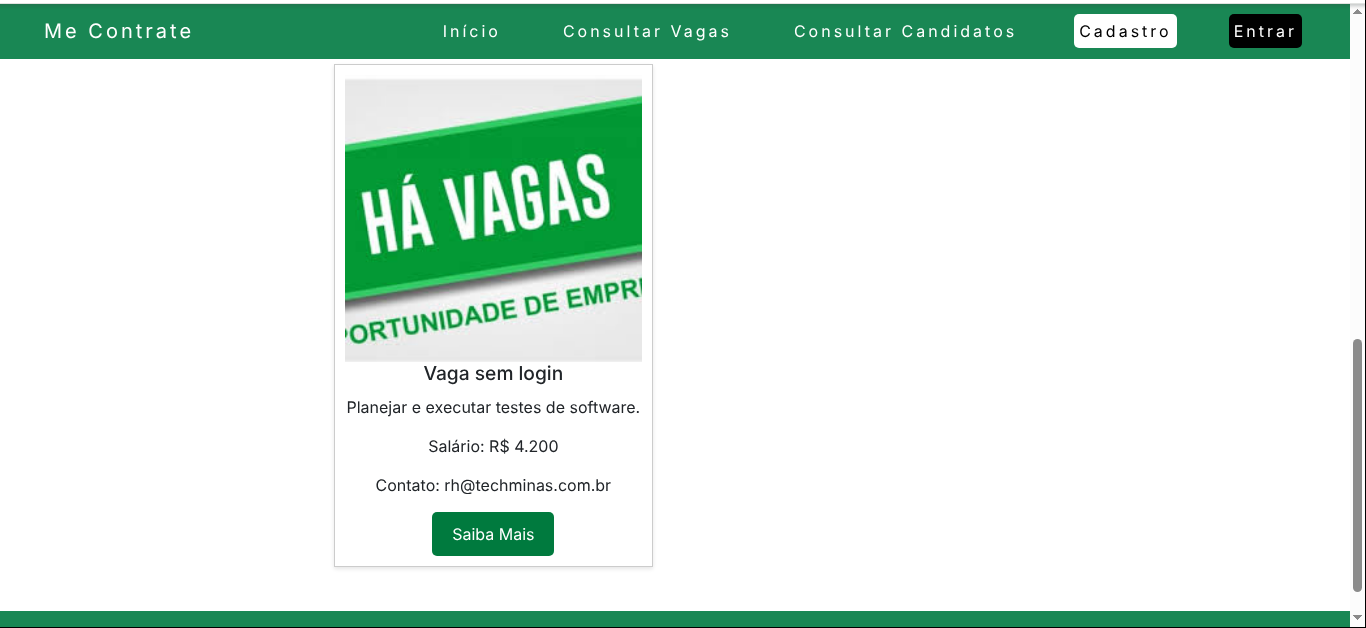
\includegraphics[width=\textwidth,height=4.2cm,keepaspectratio]{CT30_c_vaga_publicada.png}\\
      \scriptsize\textbf{CT30:} visitante \textbf{sem login} publica uma vaga.
    \end{column}
    \hfill
    \begin{column}{0.49\textwidth}
      \centering
      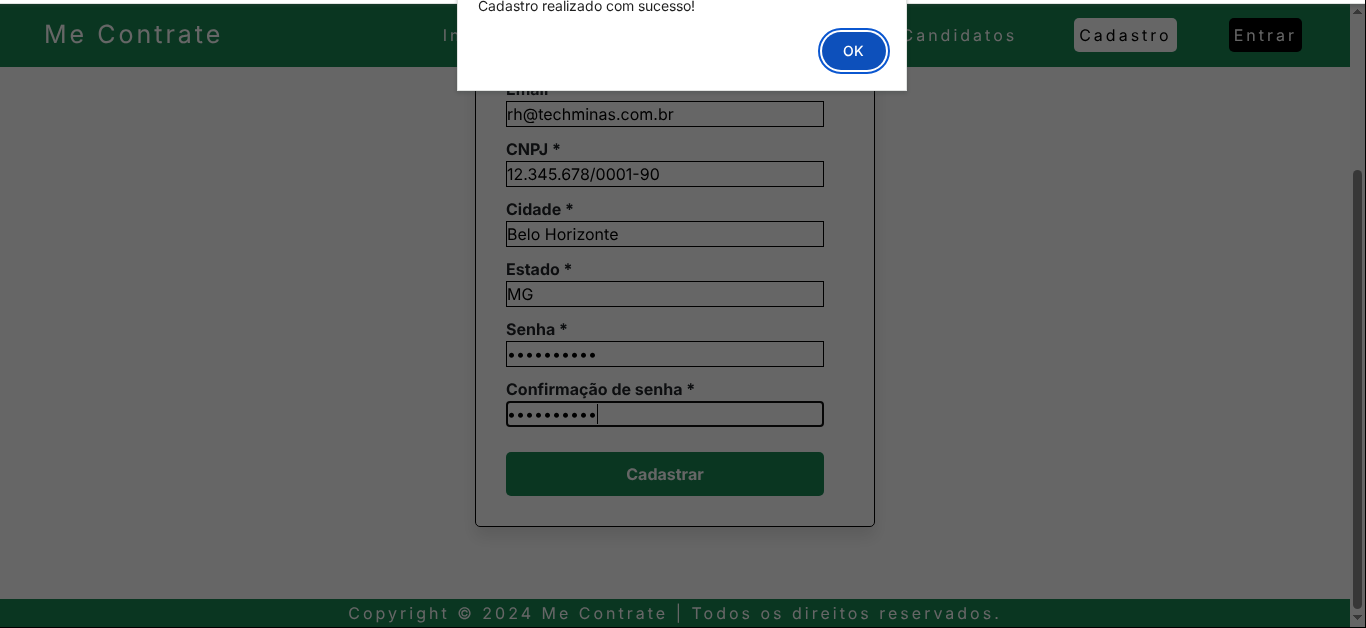
\includegraphics[width=\textwidth,height=4.2cm,keepaspectratio]{CT24_b_alerta.png}\\
      \scriptsize\textbf{CT24:} empresa cadastrada com \textbf{e-mail repetido}.
    \end{column}
  \end{columns}
  \vspace{2mm}
  \small Também reprovados: \textbf{CT22} (modal sem a empresa) e \textbf{CT26} (sair sem mensagem).
  Aprovados: navegação, detalhes do candidato, perfil, acesso sem login, limpar vagas e celular.
\end{frame}

\begin{frame}{Relatório de Defeitos}{10 defeitos, 5 de severidade alta}
  \scriptsize
  \begin{tabular}{@{}l l l p{5.6cm} p{4.6cm}@{}}
    \toprule
    \textbf{ID} & \textbf{Caso} & \textbf{Sev.} & \textbf{Defeito} & \textbf{Solução proposta} \\
    \midrule
    D01 & CT20 & Alta & Vagas cadastradas sem id único & Gerar id no cadastro \\
    D03 & CT10 & Alta & \texttt{atualizarBotoes} lança exceção & Refatoração 2 \\
    D05 & CT24 & Alta & E-mail duplicado aceito & Verificar antes de gravar \\
    D07 & CT30 & Alta & Cadastro de vaga sem login & Exigir sessão de empresa \\
    D10 & CT11 & Alta & Senhas em texto puro (LGPD) & Back-end com hash \\
    \midrule
    D02 & CT06 & Média & Mensagem cita o campo errado & Corrigir texto e ids \\
    D04 & CT22 & Média & Modal não mostra a empresa & Preencher \texttt{modalInfo} \\
    D06 & CT26 & Média & Sair sem mensagem e link quebrado & Um único tratador \\
    D09 & Revisão & Média & Login sobrescreve o usuário & Refatoração 1 \\
    D08 & CT23 & Baixa & Erro no console e título errado & Corrigir guarda e título \\
    \bottomrule
  \end{tabular}
\end{frame}

\begin{frame}{Resultado Geral}{30 casos executados}
  \begin{columns}[c,onlytextwidth]
    \begin{column}{0.48\textwidth}
      \centering
      \begin{tabular}{@{}lccc@{}}
        \toprule
        \textbf{Técnica} & \textbf{Casos} & \textbf{OK} & \textbf{Falha} \\
        \midrule
        Unidade & 10 & 8 & 2 \\
        Selenium & 10 & 9 & 1 \\
        Manual & 10 & 6 & 4 \\
        \midrule
        \textbf{Total} & \textbf{30} & \textbf{23} & \textbf{7} \\
        \bottomrule
      \end{tabular}
    \end{column}
    \hfill
    \begin{column}{0.48\textwidth}
      \begin{block}{Conclusões}
        \small
        \begin{itemize}
          \item Os fluxos principais funcionam.
          \item Os problemas estão em \textbf{controle de acesso}, \textbf{validação} e \textbf{código duplicado}.
          \item As refatorações eliminam 2 defeitos sem mudar o comportamento.
        \end{itemize}
      \end{block}
    \end{column}
  \end{columns}
\end{frame}

\begin{frame}[plain]
  \centering
  \vspace{1.2cm}
  {\Huge\color{pucazul}\textbf{Obrigado!}}\\[6mm]
  {\large Perguntas?}\\[8mm]
  \small
  \textbf{Repositório de testes:} {\footnotesize \href{https://github.com/otavio-castro/projeto-testes-sistema-rh}{github.com/otavio-castro/projeto-testes-sistema-rh}}\\[1mm]
  \textbf{TI original:} {\footnotesize github.com/ICEI-PUC-Minas-PBE-ADS-TI/pbe-si-ads-2024-2-tiaw-t1-sistema-de-rh}\\[8mm]
  
\includegraphics[height=1.3cm]{logo_puc_azul.png}
\end{frame}

\end{document}
